\documentclass[journal=jacsat,manuscript=article]{achemso}
\usepackage[version=3]{mhchem}
\usepackage{amsmath}
\newcommand*\mycommand[1]{\texttt{\emph{#1}}}
\author{Claire Gillespie}
\affiliation{Department of Chemistry and Chemical Biology, McMaster
University, 1280 Main Street West, Hamilton, ON, L8S 4L8}
\email{gillec1@mcmaster.ca}
\phone{226-232-4613}

\abbreviations{MSI-CE-MS, CUD, FTND}

\keywords{tobacco, cannabis, biomarker, metabolome, drugs of abuse}

\title[An \textsf{achemso} demo]{Biochemical verification of tobacco and
cannabis smoking status and dependence via characterization of salivary
metabolome}
\makeatletter
\ifxetex
  \usepackage[setpagesize=false, % page size defined by xetex
              unicode=false, % unicode breaks when used with xetex
              xetex]{hyperref}
\else
  \usepackage[unicode=true]{hyperref}
\fi
\hypersetup{breaklinks=true,
            bookmarks=true,
            pdfauthor={},
            pdftitle={},
            colorlinks=true,
            urlcolor=blue,
            linkcolor=magenta,
            pdfborder={0 0 0}}
\urlstyle{same}  % don't use monospace font for urls


% tightlist command for lists without linebreak
\providecommand{\tightlist}{%
  \setlength{\itemsep}{0pt}\setlength{\parskip}{0pt}}




\begin{document}
\begin{abstract}
Cannabis and tobacco are two of the most widely consumed narcotics
globally and pose significant harms from smoke exposures, including
chronic disease burden, drug addiction and/or cognitive impairment in
vulnerable populations. Current methods that assess nicotine or cannabis
dependence rely solely on standardized questionnaires that are prone to
bias and misreporting. Thus, there is a need for an objective and
non-invasive approach for the assessment of smoking status. Herein we
introduce a high-throughput method for characterizing the salivary
metabolome from a cohort of participants involved in a Trier Social
Stress Test to examine how smoking and cannabis use affect cognition.
Following a sample workup of diluted saliva filtrate, targeted profiling
of the salivary metabolome was conducted using multisegment
injection-capillary electrophoresis mass-spectrometry (MSI-CE-MS) with
full-scan data acquisition. Multivariate and univariate statistical
analyses of saliva samples will result in the identification of
biomarkers associated with smoking status when comparing self-reported
non-smokers (n=12), cannabis only (n=36), and cannabis-tobacco users
(n=15). Temporal changes in the salivary metabolome will be explored by
MSI-CE-MS prior to and following standardized psychosocial stress
experiments among participants to identify biomarkers associated with
cognitive dysfunction. This method will confirm recent exposure to other
drugs of abuse that may confound behavioral responses to psychosocial
stress and not captured by standardized questionnaires, including
nicotine, opioids and benzodiazepenes. This research will elucidate the
underlying mechanisms of stress intolerance among cannabis users while
identifying salivary biomarkers associated with cannabis and tobacco
dependence, including screening for concomitant use of other drugs prone
to abuse.
\end{abstract}
\begin{tocentry}
Some journals require a graphical entry for the Table of Contents.
This should be laid out ``print ready'' so that the sizing of the
text is correct.

Inside the \texttt{tocentry} environment, the font used is Helvetica
8\,pt, as required by \emph{Journal of the American Chemical
Society}.

The surrounding frame is 9\,cm by 3.5\,cm, which is the maximum
permitted for  \emph{Journal of the American Chemical Society}
graphical table of content entries. The box will not resize if the
content is too big: instead it will overflow the edge of the box.

This box and the associated title will always be printed on a
separate page at the end of the document.
\end{tocentry}

\hypertarget{study-motivation}{%
\section{Study Motivation}\label{study-motivation}}

Cannabis and tobacco are among the top three most prevalent drugs used
globally, with 2.5\% and 22.3\% of the global population consuming
cannabis and tobacco in 2020.\textsuperscript{1,2} Cause for concern
arises given tobacco smoking remains the primary cause of preventable
death in Canada, with 17\% of smoking related deaths being caused by
cancers, cardiovascular and respiratory diseases.\textsuperscript{3}
Moreover, smoking poses a serious financial burden on the Canadian
health care system, with the total costs of tobacco use being \$16.2
billion in 2012.\textsuperscript{4} Furthermore, cannabis has become the
second most commonly used drug of abuse after alcohol in Canada, notably
among young adults. According to the 2021 Canadian cannabis survey, 37\%
and 49\% of consumers are ages 16-19 and 20-24, respectively with 19\%
reporting the intake of marijuana on a daily basis.\textsuperscript{5}
With this rampant increase in cannabis use among young Canadian adults,
there is growing concern on the prevalence of cannabis use disorder
since it can contribute to addiction with deleterious psychiatric
effects that impair normal cognitive function.\textsuperscript{6}
Specifically, prolonged, and frequent use of cannabis can alter brain
circuitry wherein individuals may experience distress intolerance
disorder, which is the inability to experience unpleasant, adverse, or
uncomfortable emotions.\textsuperscript{7} With both cannabis and
tobacco use raising concerns in terms of the physical and mental harms
among vulnerable populations, there is a need to determine the
susceptibility an individual may have in depending on these narcotics.
However, current methods for the assessment of nicotine or cannabis
dependence rely solely on standardized questionnaires that are prone to
bias and misreporting. Clinicians would thus benefit from a non-invasive
yet objective identification of cannabis and tobacco smoking status
while examining their putative harmful effects to better guide more
personalized therapeutic interventions.

\hypertarget{current-methods-for-diagnosing-cannabis-and-tobacco-dependence}{%
\section{Current Methods for Diagnosing Cannabis and Tobacco
Dependence}\label{current-methods-for-diagnosing-cannabis-and-tobacco-dependence}}

In order for a clinician to determine the magnitude of dependence that
an individual may experience towards cannabis and/or tobacco, they
employ standardized tests such as the Fagerstrom Test for Nicotine
Dependence (FTND) and the Cannabis Use Disorder Identification Test
(CUDIT). The FTND test encompasses 6 questions wherein the individual
must check off their smoking habits, with the sum of their answers
resulting in an FTND score. Dependence scores can range from 0-2 being
very low, 3-5 being medium and 6-10 being very high.\textsuperscript{8}
Furthermore, the CUDIT is a questionnaire with 8 total questions where
the individuals must rank their cannabis use habits, and their resulting
sum CUDIT score is subsequently tabulated. According to literature,
individuals with CUDIT scores of 12 and below have low cannabis
dependence, whereas individuals with CUDIT scores of 13 and above
indicate a susceptibility for cannabis use disorder with the
recommendation of further intervention.\textsuperscript{9} However,
given that there are societal expectations among the population, being
that it is frowned upon to use drugs as a coping mechanism, individuals
may feel pressured to falsify their answers to these standardized tests,
resulting in lower FTND or CUDIT scores than expected. Hence, there is a
need for a biological confirmation of the self-reported information to
compliment the data obtained by standardized questionnaires. Therefore,
the goals of this study were through the characterization of the
salivary metabolome of control, cannabis, and cannabis tobacco users,
first confirm that nicotine can be considered an exogenous biomarker of
tobacco smoking status, and second identify a marker that differentiates
the sub-groups based on smoking status while reflecting the harmful
effects of habitual cannabis and/or tobacco use. Finally, investigations
on the mechanisms of cannabis use disorder will be conducted through the
analysis of individuals from the cannabis only sub-group at baseline to
determine whether there is an underlying change among individuals with
high versus low CUDIT scores.

\hypertarget{metabolomic-characterization}{%
\section{Metabolomic
Characterization}\label{metabolomic-characterization}}

To determine an individual's metabolism, the salivary metabolome of the
participants was characterized. Metabolomics is an emerging field in
functional genomics which encompasses the analysis of low molecular
weight metabolites in complex biological samples using new advances in
high resolution mass spectrometry (MS).\textsuperscript{10} The human
metabolome comprises both endogenous and exogenous metabolites
(including drugs of abuse), which are influenced by both genetic factors
and environmental exposures.\textsuperscript{11} Previous research has
proposed that the salivary metabolome may provide unique insights into
behavioral responses to psychological stress using a non-invasive
biofluid.\textsuperscript{12} Furthermore, although untargeted salivary
metabolomic studies have been applied to identify novel biomarkers
associated with cancer and oral health studies,\textsuperscript{10,13}
no report to date has examined its potential for characterizing stress
intolerance in high-risk individuals with cannabis use disorder as
compared to non-users or infrequent cannabis users not prone to
dependence. In this thesis, one will develop a robust protocol for
untargeted metabolite profiling from unstimulated saliva specimens using
multisegment injection-capillary electrophoresis-mass spectrometry
(MSI-CE-MS) as a high throughput method for biomarker discovery with
stringent quality control.\textsuperscript{14,15}

\hypertarget{instrument-methodology}{%
\section{Instrument Methodology}\label{instrument-methodology}}

Current methods for untargeted metabolite analysis include NMR and MS
coupled with chromatography, with the gold standard being liquid
chromatography-mass spectrometry (LC-MS) due to its broad coverage of
analytes with high efficiency separations, and highly selective
results.\textsuperscript{16} However, the limitations of these methods
involve the long processing times which are limited to low sample
throughput as well as the generated chromatograms may provide low
resolution peaks, making it difficult to identify metabolites as well as
the number of metabolites present in the data set.\textsuperscript{17}
In contrast, multisegment injection-capillary electrophoresis-mass
spectrometry (MSI-CE-MS) utilizes a multiplexed separation platform for
metabolomics,\textsuperscript{18} allowing for higher sample throughput,
improved quality control and lower sample volume
requirements.\textsuperscript{19} This method employs an isocratic
aqueous buffer with a coaxial sheath liquid interface to provide a
homogenous solution for electromigration and ionization under steady
state conditions,\textsuperscript{14} with customized serial injections
accelerating the potential for biomarker discovery and robust
inter-batch adjustment possible for use in large scale metabolomic
studies.\textsuperscript{20} Data acquisition using MSI-CE-MS first
involves injecting 13 samples each separated by the same volume
background electrolyte (BGE) spacer into the capillary (Figure 1). The
application of a voltage initiates the flow of analytes from the
injection site to the electrospray ionization (ESI) source on the
time-of-flight mass spectrometer (TOF-MS). This gentle ionization source
uses electrical energy to assist the transfer of ions from solution to
the gaseous phase through protonation in positive mode and deprotonation
in negative mode.\textsuperscript{21} Analytes are subsequently
separated by their mass and charge using an untargeted full-scan
approach in the TOF-MS. A full-scan data acquisition total ion
electropherogram (TIE) is the result of one run in MSI-CE-MS (Figure 2).
From the TIE, one can extract the m/z of metabolites of interest in a
targeted manner, which generates extracted ion electropherograms (EIE)
for both positive and negative mode (Figures 3 \& 4). Each EIE should
show thirteen peaks pertaining to the 13 injections from the capillary.
In order to confirm a metabolites identity, one can refer to its mass
spectrum (Figure 5), where a prominent molecular ion peak should be
present at the same mass to charge (m/z) as the metabolite, as well as a
less prominent C-13 peak approximately one mass unit away. Further
confirmation can be given when examining the mass resolution of the
metabolite of interest (Figure 5). Finally, MSI-CE-MS provides the
ability to have a quality control sample in each run, whose relative
peak areas (RPAs) are compared to monitor the performance of the
platform and any potential instrumental drift.

\hypertarget{future-work}{%
\section{Future Work}\label{future-work}}

Future work will involve the statistical analysis of the various
metabolites of interest found through data processing the 206 biological
samples and 18 pooled quality control samples. Trends within the three
sub-groups of individuals, being control, cannabis users, and
cannabis-tobacco users, will be investigated pre and post the Trier
Social Stress Test to determine whether their salivary metabolomes can
be differentiated at baseline, or whether the stress test affects one
group significantly. Further analysis of cannabinoid content will
follow, using LC-MS to confirm that salivary cannabinoids can be
exogenous biomarkers for cannabis use while also providing more insight
on cannabis dependence through the complimentary relation with reported
CUDIT scores.

\hypertarget{supplementary-information}{%
\section{Supplementary Information}\label{supplementary-information}}

\hypertarget{references}{%
\subsection{References}\label{references}}

\begin{enumerate}
\def\labelenumi{\arabic{enumi}.}
\item
  Cannabis. (2023). World Health Organization.
\item
  Tobacco. (2023). World Health Organization.
\item
  (2011). Smoking and Mortality. Canada.ca. Government of Canada.
\item
  (2017). The Costs of Tobacco Use in Canada, 2012. Canada.ca.
  Government of Canada.
\item
  \begin{enumerate}
  \def\labelenumii{(\arabic{enumii})}
  \setcounter{enumii}{2020}
  \tightlist
  \item
    Canadian Cannabis Survey 2021: Summary. Canada.ca. Government of
    Canada.
  \end{enumerate}
\item
  Patel, J., \& Marwaha, R. (2022) Cannabis use disorder. Eng. J. Med.
\item
  Volkow, N. D., Baler, R. D., Weiss, S. R. B., \& Compton, W. M.

  \begin{enumerate}
  \def\labelenumii{(\arabic{enumii})}
  \setcounter{enumii}{2013}
  \tightlist
  \item
    Adverse health effects of marijuana use. Eng. J. Med. 370 (23),
    2219-2227.
  \end{enumerate}
\item
  Lim, K.H., The, C.H., Lim, H.L., Khoo, Y.Y., Lau, K.J., Yy, C., Mohd
  Ghazalig, S., Kee Cc, C.C., Lim, K.K., Ibrahim, N., and Yusoff, F.M.
  (2016). Reliability and Validity of the Fagerstrom Test for Cigarettes
  Dependence among Malaysian Adolescents. Iran J Public Health.
  45(1):104-5.
\item
  Bonn-Miller, M.O., Heinz, A.J., Smith, E.V., Bruno, R., and Adamson,
  S. (2016). Preliminary Development of a Brief Cannabis Use Disorder
  Screening Tool: The Cannabis Use Disorder Identification Test
  Short-Form. Cannabis Cannabinoid Res. 1 (1):252-261.
\item
  Liebsch, C., Pitchika, V., Pink, C., Samietz, S., Kastenmüller, G.,
  Artati, A., Suhre, K., Adamski, J., Nauck, M., Völzke, H., Friedrich,
  N., Kocher, T., Holtfreter, B., \& Pietzner, M. (2019). The Saliva
  Metabolome in Association to Oral Health Status. J. of Dent. Res. 98
  (6), 642--651.
\item
  Patti G. J., Yanes O., \& Siuzdak G. 2012. Innovation: metabolomics:
  the apogee of the omics trilogy. Nat. Rev.~Mol. Cell. Biol. 13 (4),
  263--269.
\item
  Gardner, A., Carpenter, G., \& So, P. W. (2020). Salivary
  metabolomics: From diagnostic biomarker discovery to investigating
  biological function. Metab. 10 (2).
\item
  Kuwabara, H., Katsumata, K., Iwabuchi, A., Udo, R., Tago, T.,
  Kasahara, K., Mazaki, J., Enomoto, M., Ishizaki, T., Soya, R., Kaneko,
  M., Ota, S., Enomoto, A., Soga, T., Tomita, M., Sunamura, M.,
  Tsuchida, A., Sugimoto, M., \& Nagakawa, Y. (2022). Salivary
  metabolomics with machine learning for colorectal cancer detection.
  Canc. Sci. 113 (9), 3234--3243.
\item
  DiBattista, A., Rampersaud, D., Lee, H., Kim, M., \& Britz-McKibbin,
  P. (2017). High Throughput Screening Method for Systematic
  Surveillance of Drugs of Abuse by Multisegment Injection--Capillary
  Electrophoresis--Mass Spectrometry. J. Anal. Chem. 89 (21),
  11853-11861.
\item
  Shanmuganathan M., Macklai S., Barrenas Cárdenas C., Kroezen Z., Kim
  M., Zizek W., Lee H., \& Britz-McKibbin P. (2019). High-throughput and
  Comprehensive Drug Surveillance Using Multisegment Injection-capillary
  Electrophoresis Mass Spectrometry. J. Vis. Exp. (146).
\item
  Fraisier-Vannier, O., Chervin, J., Cabanac, G., Puech, V., Fournier,
  S., Durand, V., Amiel, A., André, O., Benamar, O. A., Dumas, B.,
  Tsugawa, H., \& Marti, G. (2020). MS-CleanR: A Feature-Filtering
  Workflow for Untargeted LC-MS Based Metabolomics. Analytical
  Chemistry, 92(14), 9971--9981.
\item
  Azab, S., Ly, R., \& Britz-Mckibbin, P. (2019). Robust Method for
  High-Throughput Screening of Fatty Acids by Multisegment
  Injection-Nonaqueous Capillary Electrophoresis-Mass Spectrometry with
  Stringent Quality Control. Analytical Chemistry, 91(3), 2329--2336
\item
  Kuehnbaum, N. L., Kormendi, A., and Britz-McKibbin, P. (2013).
  Multisegment Injection-Capillary Electrophoresis-Mass Spectrometry: a
  High-Throughput Platform for Metabolomics with High Data Fidelity.
  Anal. Chem. 85, 10664--10669. \url{doi:10.1021/ac403171u}
\item
  Nori de Macedo, A., Mathiaparanam, S., Brick, L., Keenan, K., Gonska,
  T., Pedder, L., et al.~(2017). The Sweat Metabolome of Screen-Positive
  Cystic Fibrosis Infants: Revealing Mechanisms beyond Impaired Chloride
  Transport. ACS Cent. Sci. 3, 904--913.
  \url{doi:10.1021/acscentsci.7b00299}
\item
  Shanmuganathan, S., Kroezen, Z., Gill, B., Azab, S., de Souza, R. J.,
  Teo, K. K., et al.~(2021). The Maternal Serum Metabolome by
  Multisegment Injection-Capillary Electrophoresis-Mass Spectrometry: A
  Standardized Data Workflow for Large- Scale Epidemiological Studies.
  Nat. Prot. 16, 1966--1994. \url{doi:10.1038/s41596-} 020-00475-0
\item
  Ho, C.S., Lam, C.W., Chan, M.H., Cheung, R.C., Law, L.K., Lit, L.C.,
  Ng, K.F., Suen, M.W., and Tai, H.L. (2003). Electrospray ionisation
  mass spectrometry: principles and clinical applications. Clin Biochem
  Rev.~24(1):3-12.
\end{enumerate}

\hypertarget{figures}{%
\subsection{Figures}\label{figures}}

\begin{figure}
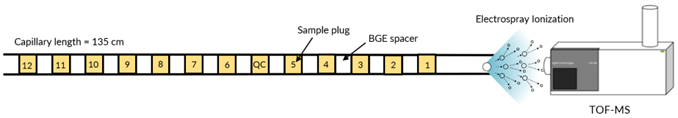
\includegraphics[width=1\linewidth]{../Figures/Figure1} \caption{Figure 1. Visualization of an injection sequence used in MSI-CE-MS. Thirteen samples are injected hydrodynamically to the capillary, each separated by the same volume background electrolyte spacer that is injected electrokinetically. A voltage applied to the capillary transports the injections to the electrospray ionization source where metabolites are protonated (in positive mode) or deprotonated (in negative mode). Full-scan data acquisition of the salivary metabolome is done using the time-of-flight mass spectrometer.}\label{fig:unnamed-chunk-1}
\end{figure}

\begin{figure}
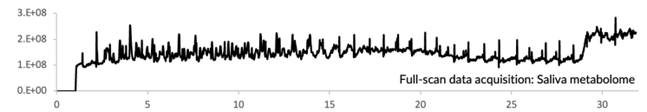
\includegraphics[width=1\linewidth]{../Figures/Figure2} \caption{Figure 2. Total ion electropherogram (TIE) of a full-scan data acquisition of the salivary metabolome. TIE shows all features from the entire run versus time. Each run was approximately 32 minutes total.}\label{fig:unnamed-chunk-2}
\end{figure}

\begin{figure}
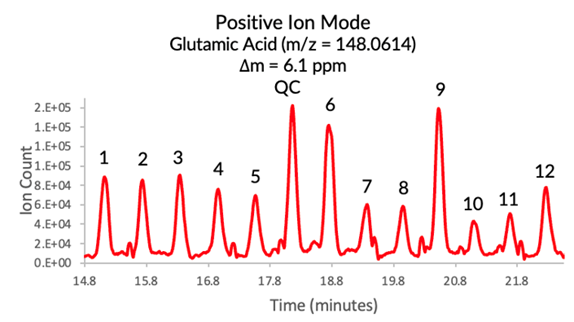
\includegraphics[width=1\linewidth]{../Figures/Figure3} \caption{Figure 3. Extracted ion electropherogram (EIE) of glutamic acid in positive mode. EIE shows 13 peaks total pertaining to the injection sequence in Figure 1. The variation shown in relative peak area of the injections is likely due to natural biological variation.}\label{fig:unnamed-chunk-3}
\end{figure}

\begin{figure}
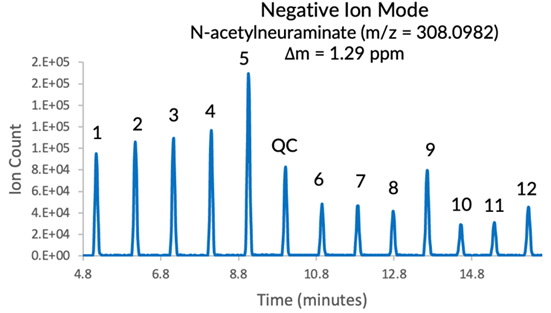
\includegraphics[width=1\linewidth]{../Figures/Figure4} \caption{Figure 4. Extracted ion electropherogram (EIE) of N-acetylneuraminate in negative mode. EIE shows 13 peaks total pertaining to the injection sequence in Figure 1. The variation shown in relative peak area of the injections is likely due to natural biological variation.}\label{fig:unnamed-chunk-4}
\end{figure}

\begin{figure}
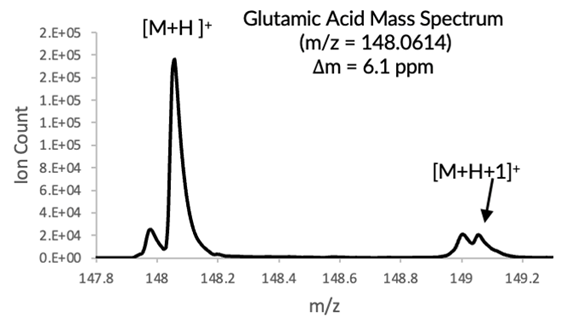
\includegraphics[width=1\linewidth]{../Figures/Figure5} \caption{Figure 5. Mass spectrum of glutamic acid in positive mode. Mass spectrums are used to confirm a metabolites identity, shown by a prominent molecular ion ([M+H]+) peak at the metabolites m/z as well as a less prominent C-13 peak ([M+H+1]+) approximately one mass unit away. Further confirmation of its identity can be shown in examining its small resolution.}\label{fig:unnamed-chunk-5}
\end{figure}
\end{document}
